\documentclass[aps,twocolumn,showpacs,floatfix,nofootinbib,preprintnumbers,superscriptaddress,amsmath,amssymb]{revtex4-1}
\usepackage{graphicx}
\usepackage{epsfig}
\usepackage{bm}
\usepackage{color}
\usepackage{float}
\usepackage{dcolumn}
\usepackage{multirow} 
\usepackage{subfigure}

\newcommand{\Ho}{\hat{H}^{\rm od}}
\newcommand{\expec}[1]{\langle #1 \rangle}
\DeclareMathOperator\erf{erf}
\DeclareMathOperator\erfc{erfc}

\begin{document}

\title{Many-body approaches to the homogeneous electron gas in two and three dimensions} 


\author{Justin G.~Lietz}
\affiliation{National Superconducting
  Cyclotron Laboratory and Department of Physics and Astronomy, Michigan State University, East Lansing, MI 48824, USA} 

\author{Scott K.~Bogner}
\affiliation{National Superconducting
  Cyclotron Laboratory and Department of Physics and Astronomy, Michigan State University, East Lansing, MI 48824, USA} 

\author{Morten Hjorth-Jensen} 
\affiliation{National Superconducting Cyclotron
  Laboratory and Department of Physics and Astronomy, Michigan State University, East Lansing, MI 48824, USA}
\affiliation{Department of Physics, University of Oslo, N-0316 Oslo, Norway} 

\begin{abstract} 
We present results for the two- and three-dimensional homogeneous
electron gas using first principle methods like coupled cluster
theory and two recently developed methods, the in-medium Similarity Renormalization. In particular, we present
new results for the correlation energy for the two-dimensional
electron gas and analyze our results in terms of finite size effects and basis functions.
\end{abstract}

\pacs{02.70.Ss, 31.15.A-, 31.15.bw, 31.15.V-, 71.10.Ca, 71.15.-m}

\maketitle

\section{Introduction}
A proper understanding of the role of correlations beyond a mean-field
description is of great importance for quantum many-particle
theories. For all possible quantum-mechanical systems, either finite
ones or infinite systems like the homogeneous electron gas in two or
three dimensions or nuclear or neutron star matter, the concept of an
independent particle motion continues to play a fundamental role in
studies of many-particle systems.  Deviations from such an independent
particle, or mean-field, picture have normally been interpreted as a
possible measure of correlations.  The latter are expected to reveal
important features of both the structure and the dynamics of a
many-particle system beyond a mean-field approximation.

The homogeneous electron gas is one of the few examples of a system of many
interacting particles that allows for a solution of the mean-field
Hartree-Fock equations on a closed form.  To first order in the
electron-electron interaction, this applies to ground state properties
like the energy and its pertinent equation of state as well.  The
homogeneus electron gas is a system of electrons that is not
influenced by external forces except by an attraction provided by a
uniform background of ions. These ions give rise to a uniform
background charge.  The ions are stationary and the system as a whole
is neutral.
Irrespective of this simplicity, this system, in both two and
three-dimensions, has eluded a proper description of correlations in
terms of various first principle methods, except perhaps for quantum
Monte Carlo methods. In particular, the diffusion Monte Carlo
calculations of Ceperley {\em et al.}
\cite{ceperley1980,tanatar1989}, are presently still considered as the
best possible benchmarks for the two- and three-dimensional electron
gas. 

The electron gas, in 
two or three dimensions is thus interesting as a test-bed for 
electron-electron correlations. The three-dimensional 
electron gas is particularly important as a cornerstone 
of the local-density approximation in density-functional 
theory. In the physical world, systems 
similar to the three-dimensional electron gas can be 
found in, for example, alkali metals and doped 
semiconductors. Two-dimensional electron fluids are 
observed on metal and liquid-helium surfaces, as well as 
at metal-oxide-semiconductor interfaces. However, the Coulomb 
interaction has an infinite range, and therefore 
long-range correlations play an essential role in the
electron gas. At low densities, the electrons become 
localized and form a lattice. This so-called Wigner 
crystallization \cite{wigner1934} is a direct consequence 
of the long-ranged repulsive interaction. At higher
densities, the electron gas is better described as a
liquid \cite{ceperley1978,ceperley1980,tanatar1989,bishop1982}. 
When using, for example, Monte Carlo methods 
\cite{foulkes2001}, the electron gas must be approximated 
by a finite system. The long-range Coulomb interaction 
in the electron gas causes additional finite-size effects 
\cite{fraser1996,chiesa2006,drummond2008} that are not
present in other infinite systems like nuclear matter or neutron star matter in 
\cite{hagen2014}. 
This poses additional challenges to many-body methods when applied 
to the electron gas.

The aim of this work is to present results for the infinite electron
gas using several many-body methods.  We focus in particular on
coupled-cluster theory (add ref), the recently develop in-medium
similarity renormalization group methods, full-configuration
interaction quantmum Monte Carlo \cite{booth2009,shepherd2012a,booth2013}
We present results for all these methods and study in particular both finite size effects and effects due to
a truncation in the single-particle basis (add more refs). 

More 

\section{Formalism}
\label{sec:formalism}

\subsection{Previous studies of the electron gas}

The electron gas has been studied using a large number 
of different approaches, and we will here only mention
some of the most important works that are relevant here. 
We start with the three-dimensional electron 
gas, which has got most attention in the literature.
The three-dimensional electron gas will mainly serve as a benchmark for our calculations,

It is a well-kown fact that the correlation energy
of the three-dimensional electron gas diverges 
at second order in perturbation theory. The particle-hole ring diagrams 
dominate at the limit of high density. Even though
all these diagrams diverge when calculated separately,
the energy converges when summing all direct 
particle-hole ring diagrams to infinite order.
Gell-Mann and Brueckner obtained for this so-called
random-phase approximation (RPA) the first terms of
the exact energy in the high-density limit 
\cite{gellmann1957}. 


At metallic and lower densities, short-ranged correlations
become significant. Singwi \emph{et al.} \cite{singwi1968}
and Lowy and Brown \cite{lowy1975} came up with early attempts 
to combine RPA with contributions for short-ranged 
correlations. The calculations of Singwi \emph{et al.}
were based on dielectric function theory, whereas Lowy and
Brown interpolated between short- and long-range models
using a diagrammatic technique. 

In 1978, Ceperley used \cite{ceperley1978} 
the variational Monte Carlo (VMC) method to 
study the two- and three-dimensional electron gas. The
obtained VMC ground-state energies were shown to be close
to other results at that time. Higher accuracy can be obtained with
the diffusion Monte Carlo (DMC) method (in nuclear physics,
this method is commonly named Green's function Monte Carlo). 
The DMC results of Ceperley and Alder from 1980 
\cite{ceperley1980} are still, more than thirty years later, 
among the most accurate energy estimates for the 
three-dimensional electron gas. In Ref.~\cite{ceperley1980},
the fermion sign problem is handled using 
a released-node approximation. Similar accuracy has been 
obtained in more recent calculations using the 
backflow-correlation technique \cite{kwon1998}, which is used 
to relax the simpler fixed-node approximation. 

When modelling the electron gas using a finite box, as is
commonly done in Monte Carlo methods, the energy has an error
compared to the electron gas at the thermodynamic limit. 
At the thermodynamic limit, plane-wave single-particle states
fill the Fermi sphere with a continuous spectrum. When the
system is approximated using a finite box, the 
single-particle spectrum becomes discrete. This 
discretization gives an 
error that is common to systems with short-ranged and 
long-ranged interactions. The perhaps most obvious way to
correct for finite-size effects related to a discrete 
single-particle basis, is by using an extrapolation formula.
As is described in Ref.~\cite{drummond2008}, results from
Hartree-Fock and density-functional theory calculations 
can be used to construct extrapolation methods. Another
approach that efficiently reduces the finite-size error
is a technique that utilizes so-called twisted boundary 
conditions \cite{lin2001}. Twisted boundary conditions 
means that the single-particle wave function is 
multiplied by a complex phase factor when moving from one 
simulation cell to a neighbouring cell. When averaging
over results obtained with different twist angles, the
energy estimates become much more accurate than when
using periodic boundary conditions \cite{lin2001}. 


Finite-size approximations of extended Coulombic systems, 
such as the electron gas, have additional errors that are 
caused by the long-ranged interaction \cite{fraser1996,chiesa2006,drummond2008}. 
Interactions with electrons in
neighbouring cells can be summed using, for example,
Ewald's method \cite{ewald1921,fraser1996,wood2004,drummond2008}. In 
Ewald's approach, each electron in the simulation cell
interacts with an infinite number of image charges located
at the same local position in all other cells. As is shown 
in Refs.~\cite{fraser1996,chiesa2006}, 
Ewald's interaction cannot describe the exchange-correlation
energy correctly. Chiesa \emph{et al.} \cite{chiesa2006}
used a static structure factor and a Jastrow factor
derived from RPA to estimate the correction to Ewald's
method. The correction technique of Chiesa \emph{et al.}
is directly applicable only to Monte Carlo methods.
Fraser \emph{et al.} \cite{fraser1996} suggested two 
different effective interactions that avoid the screening 
effects caused by Ewald's interaction . The most successful
alternative was to use a normal Coulomb interaction combined 
with the minimum-image convention \cite{fraser1996}.
The reader is referred to Ref.~\cite{drummond2008} for
more details about finite-size effects and different
approaches to correct for the related errors.


The full configuration-interaction quantum Monte Carlo 
(FCIQMC) met\-hod \cite{booth2009} is a new approach to the 
quantum many-body problem, in which the full 
configuration-interaction (FCI) equations \cite{harris1992} are 
solved approximately using a Monte Carlo technique. Similarly 
as in the DMC or GFMC methods, the Schr{\"o}dinger equation is 
written as a diffusion equation with an imaginary time 
variable \cite{shepherd2012a}. In the FCI method, the total 
wave-function ansatz 
is expressed as a linear combination of Slater determinants 
constructed from a given single-particle basis. In FCIQMC, 
the coefficients in the expansion of Slater determinants 
are obtained as the large-time limit of a random walk 
\cite{shepherd2012a}. As we discussed above, Monte Carlo
calculations of the electron gas have an error related to 
the finite number of particles in the simulation cell. 
Methods such as FCIQMC, CC, and partial summations derived 
from many-body perturbation theory have and additional error 
when studying systems with a discrete single-particle basis: 
The result depends on the given set of both occupied and 
unoccupied single-particle states \cite{shepherd2012b}. 
This error can be corrected for by using, for example, the 
single-point extrapolation technique \cite{shepherd2012b,
shepherd2012c} introduced by Shepherd \emph{et al.} The 
FCIQMC method has recently been applied to finite 
electron-gas systems \cite{shepherd2012a,shepherd2012b,
shepherd2012c}, giving results in close agreement
with DMC calculations utilizing backflow correlations 
\cite{shepherd2012a}. 

Singal and Das \cite{singal1973} were the first to study 
the electron gas using a CC approach. The approximation
they used is similar to the BHF method \cite{haftel1970}, 
and does not properly include particle-hole ring diagrams.
Later, Freeman did CC calculations \cite{freeman1977} in 
which only ring diagrams and their exchange parts were 
retained in a CC doubles approximation. The results of both
Singal and Das \cite{singal1973} and Freeman 
\cite{freeman1977} compared well with dielectric-function
approaches. Presently, the most accurate CC caclulations of 
the three-dimensional electron gas are those of Bishop and
L{\"u}hrmann \cite{bishop1978,bishop1982}. Bishop and
L{\"u}hrmann derived a CC SUB2 approximation (also called
CC doubles (CCD) \cite{shavittbartlett2009}) for the electron gas, 
extended with some ladder contributions from higher-order
amplitudes. As the authors describe in 
Ref.~\cite{bishop1978}, the CCD approximation 
contains many more diagrammatic classes than
partial-summation techniques derived from perturbation 
theory. The CCD approximation takes account of 
particle-particle and hole-hole ladders, particle-hole
ring diagrams including exchange terms, and many other
diagrams to infinite order in perturbation theory. 
In their CC approximations, Bishop and L{\"u}hrmann 
replaced summations over hole states by averages. In
fact, the nine-dimensional CC amplitudes were simplified
to one-dimensional objects, with the absolute value
of the transfer momentum being the only variable. 
The authors showed that the state-average approximation
is accurate in the RPA approximation.
Bishop and L{\"u}hrmann neglected some diagrammatic 
classes, such as the hole-hole ladders and mixed ladders, 
which they assumed to be small. Despite all these 
approximations, the final CC energies are very accurate 
in a typical metallic density range. Relative 
differences of less than one percent
compared to DMC calculations of Ceperley and Alder
may indicate that the extended CCD approximation describes
most of the relevant correlations in the three-dimensional
electron gas \cite{bishop1982}. 

The CC study of Bishop and L{\"u}hrmann was very successful, but still
the calculations are based on a large number of approximations. It
would be desireable to apply CC theory to the electron gas without the
same approximations.  Recently, Shepherd \emph{et al.}
\cite{shepherd2012b,shepherd2013a,shepherd2013b,shepherd2013c} have
taken up again the CC effort for the three-dimensional electron
gas. The CC calculations for the electron gas from the 1970s and 1980s
were all done at the thermodynamic limit
\cite{singal1973,freeman1977,bishop1978,bishop1982}. Unfortunately,
singularities related to the Coulomb two-body interaction may
complicate numerical calculations at the thermodynamic limit.
Shepherd \emph{et al.} approximate the electron gas using finite cubic
boxes
\cite{shepherd2012b,shepherd2013a,shepherd2013b,shepherd2013c}. When
using finite-size systems, the CC equations are simpler and most of
the problems with ill-bahaved functions are avoided.  Instead, one has
to deal with errors related to finite particle numbers and
single-particle bases, similarly as in the FCIQMC method
\cite{shepherd2012a,shepherd2012b,shepherd2012c}.


Let us finally turn our attention to the two-dimensional
electron gas. The two-dimensional electron gas is defined
in the same way as the three-dimensional counterpart, and 
similar approaches can therefore often be used to 
study both systems. As a first example, the classical 
derivation of the high-density RPA approximation by Gell-Mann 
and Brueckner \cite{gellmann1957} has been extended to the 
two-dimensional electron gas by Rajagopal and Kimball 
\cite{rajagopal1977}. 

As far as we know, the only CC calculations that have been
done for the two-dimensional electron gas are the ring
\cite{freeman1978} and particle-particle ladder \cite{freeman1983}
approximations of Freeman. Beacuse of stronger correlations
in the purely two-dimensional system, the ring approximation
was not as reliable in two dimensions as it was in the 
three-dimensional case \cite{freeman1978}. According to the 
studies of Freeman, the CC ring-diagram approximation is 
less accurate than the CC ladder approximation at 
intermediate and low densities, whereas both methods give 
similar results at the high-density limit \cite{freeman1983}.


In the earliest CC studies of the 
electron gas \cite{singal1973,freeman1977,bishop1978,
freeman1978,bishop1982,freeman1983}, the system was treated 
at the thermodynamic limit. 
Some of the most accurate calculations of the electron gas
\cite{ceperley1980,tanatar1989,shepherd2012a} have been done using finite boxes and Monte
Carlo methods. Recently, CC theory has been applied in 
several studies \cite{shepherd2012b,shepherd2013a,
shepherd2013b,shepherd2013c,roggero2013} to finite-particle 
approximations of the homogeneous electron gas. 
 Freeman has done CC studies of the two-dimensional 
electron gas including only ring \cite{freeman1978} or 
only particle-particle ladder \cite{freeman1983} diagrams 
from the CCD approximation, but to the best of our knowledge, 
nobody has done a complete CCD calculation of the 
two-dimensional homogeneous electron gas. 
As an extension of the CC calculations by Shepherd 
\emph{et al.}~\cite{shepherd2012b,shepherd2013a,shepherd2013b,shepherd2013c}
and Roggero \emph{et al.}~\cite{roggero2013}, we study
the two-dimensional electron gas in the CCD approximation
using a finite number of particles.
We validate our methods by comparing results 
for the three-dimensional electron gas with Shepherd 
\emph{et al.} \cite{shepherd2012b,shepherd2012c}.
using momentum discretized in cartesian coordinates, see discussions below. 


\subsection{Model Hamiltonian and Definitions}

The homogeneous electron gas is defined as an infinite system
consisting of electrons distributed with a constant density 
through the entire real space. The system is assumed to 
contain a constant positive background charge which cancels
the negative charges of the electrons. The Hamiltonian 
operator of the homogeneous electron gas can be written as
\cite{fetter}
\begin{align}
  \hat{H} = \hat{H}_{\text{kin}} + \hat{H}_{ee} + \hat{H}_{eb} 
  + \hat{H}_{bb},
\end{align}
where $\hat{H}_{\text{kin}}$ is the kinetic-energy operator,
$\hat{H}_{ee}$ models the electron-electron interaction,
$\hat{H}_{eb}$ represents the interaction between electrons 
and the positive background charge, and the operator 
$\hat{H}_{bb}$ gives the interaction energy of the background
charge with itself. 



Similarly as in
Refs.~\cite{shepherd2012b,shepherd2013a,shepherd2013b,shepherd2013c,roggero2013},
we approximate the homogeneous electron gas by a finite hypercube
filled with electrons. The summation over
an infinite number of Coulomb interaction terms can be efficiently
calculated using, for example, Ewald's summation technique
\cite{ewald1921,fraser1996}.  In Ewald's approach, the Coulomb
interaction is split into a short-ranged part, which is calculated
in real space, and a long-ranged part, which is summed in Fourier
space.  The kinetic energy operator is
\begin{align}
  \hat{H}_{\text{kin}} = -\frac{\hbar^{2}}{2m}\sum_{i=1}^{N}
  \nabla_{i}^{2},
\end{align}
where the sum is taken over all particles in the finite
box. The Ewald electron-electron interaction operator 
can be written as \cite{drummond2008}
\begin{align}
  \hat{H}_{ee} = \sum_{i<j}^{N} 
  v_{E}\left( \mathbf{r}_{i}-\mathbf{r}_{j}\right)
  + \frac{1}{2}Nv_{0},
\end{align}
where $v_{E}(\mathbf{r})$ is the effective two-body 
interaction and $v_{0}$ is the self-interaction, defined 
as $v_{0} = \lim_{\mathbf{r} \rightarrow 0} 
\left\{ v_{E}(\mathbf{r}) - 1/r\right\} $. The negative 
electron charges are neutralized by a positive, homogeneous 
background charge. Fraser \emph{et al.} explain 
\cite{fraser1996} how the
electron-background and background-background terms, 
$\hat{H}_{eb}$ and $\hat{H}_{bb}$, vanish
when using Ewald's interaction for the three-dimensional
electron gas. Using the same arguments, one can show that
these terms are also zero in the corresponding 
two-dimensional system. 

In the three-dimensional electron gas, the Ewald 
interaction is \cite{drummond2008}
\begin{align}
  v_{E}(\mathbf{r}) &= \sum_{\mathbf{k} \neq \mathbf{0}}
  \frac{4\pi }{L^{3}k^{2}}e^{i\mathbf{k}\cdot \mathbf{r}}
  e^{-\eta^{2}k^{2}/4} \nonumber \\
  &+ \sum_{\mathbf{R}}\frac{1}{\left| \mathbf{r}
    -\mathbf{R}\right| } \erfc \left( \frac{\left| 
    \mathbf{r}-\mathbf{R}\right|}{\eta }\right)
  - \frac{\pi \eta^{2}}{L^{3}},
\end{align}
where $L$ is the box side length, $\erfc(x)$ is the 
complementary error function, and $\eta $ is a free
parameter that can take any value in the interval 
$(0, \infty )$. The translational vector 
\begin{align}
  \mathbf{R} = L\left(n_{x}\mathbf{u}_{x} + n_{y}
  \mathbf{u}_{y} + n_{z}\mathbf{u}_{z}\right) ,
\end{align}
where $\mathbf{u}_{i}$ is the unit vector for dimension $i$,
is defined for all integers $n_{x}$, $n_{y}$, and 
$n_{z}$. These vectors are used to obtain all image
cells in the entire real space. 
The parameter $\eta $ decides how 
the Coulomb interaction is divided into a short-ranged
and long-ranged part, and does not alter the total
function. However, the number of operations needed
to calculate the Ewald interaction with a desired 
accuracy depends on $\eta $, and $\eta $ is therefore 
often chosen to optimize the convergency as a function
of the simulation-cell size \cite{drummond2008}. In
our calculations, we choose $\eta $ to be an infinitesimally
small positive number, similarly as was done in 
Refs.~\cite{shepherd2012b,shepherd2013a,shepherd2013b,shepherd2013c,roggero2013}.
This gives an interaction that is evaluated only in
Fourier space. 

When studying the two-dimensional electron gas, we
use an Ewald interaction that is quasi two-dimensional.
The interaction is derived in three dimensions, with 
Fourier discretization in only two dimensions 
\cite{wood2004}. The Ewald effective
interaction has the form \cite{wood2004}
\begin{align}
  v_{E}(\mathbf{r}) &= \sum_{\mathbf{k} \neq \mathbf{0}} 
  \frac{\pi }{L^{2}k}\left\{ e^{-kz} \erfc \left(
  \frac{\eta k}{2} - \frac{z}{\eta }\right)+ \right. \nonumber \\
  & \left. e^{kz}\erfc \left( \frac{\eta k}{2} + \frac{z}{\eta }
  \right) \right\} e^{i\mathbf{k}\cdot \mathbf{r}_{xy}} 
  \nonumber \\
  & + \sum_{\mathbf{R}}\frac{1}{\left| \mathbf{r}-\mathbf{R}
    \right| } \erfc \left( \frac{\left| \mathbf{r}-\mathbf{R}
    \right|}{\eta }\right) \nonumber \\
  & - \frac{2\pi}{L^{2}}\left\{ z\erf \left( \frac{z}{\eta }
  \right) + \frac{\eta }{\sqrt{\pi }}e^{-z^{2}/\eta^{2}}\right\},
\end{align}
where the Fourier vectors $\mathbf{k}$ and the position vector
$\mathbf{r}_{xy}$ are defined in the $(x,y)$ plane. When
applying the interaction $v_{E}(\mathbf{r})$ to two-dimensional
systems, we set $z$ to zero. Similarly as in the 
three-dimensional case, and as suggested in 
Ref.~\cite{drummond2008} for two dimensions, also here we 
choose $\eta $ to approach zero from above. The resulting 
Fourier-transformed interaction is
\begin{align}
  v_{E}^{\eta = 0, z = 0}(\mathbf{r}) = \sum_{\mathbf{k} \neq \mathbf{0}} 
  \frac{2\pi }{L^{2}k}e^{i\mathbf{k}\cdot \mathbf{r}_{xy}}. 
\end{align}
The self-interaction $v_{0}$ is a constant that can be 
included in the reference energy.


In the three-dimensional electron gas, the antisymmetrized
matrix elements are
\begin{align} \label{eq:vmat_3dheg}
  & \langle \mathbf{k}_{p}m_{s_{p}}\mathbf{k}_{q}m_{s_{q}}
  |\tilde{v}|\mathbf{k}_{r}m_{s_{r}}\mathbf{k}_{s}m_{s_{s}}\rangle_{AS} 
  \nonumber \\
  & = \frac{4\pi }{L^{3}}\delta_{\mathbf{k}_{p}+\mathbf{k}_{q},
    \mathbf{k}_{r}+\mathbf{k}_{s}}\left\{ 
  \delta_{m_{s_{p}}m_{s_{r}}}\delta_{m_{s_{q}}m_{s_{s}}}
  \left( 1 - \delta_{\mathbf{k}_{p}\mathbf{k}_{r}}\right) 
  \frac{1}{|\mathbf{k}_{r}-\mathbf{k}_{p}|^{2}}
  \right. \nonumber \\
  & \left. - \delta_{m_{s_{p}}m_{s_{s}}}\delta_{m_{s_{q}}m_{s_{r}}}
  \left( 1 - \delta_{\mathbf{k}_{p}\mathbf{k}_{s}} \right)
  \frac{1}{|\mathbf{k}_{s}-\mathbf{k}_{p}|^{2}} 
  \right\} ,
\end{align}
where the Kronecker delta functions 
$\delta_{\mathbf{k}_{p}\mathbf{k}_{r}}$ and
$\delta_{\mathbf{k}_{p}\mathbf{k}_{s}}$ ensure that the 
contribution with zero momentum transfer vanishes.
Similarly, the matrix elements for the two-dimensional
electron gas are
\begin{align} \label{eq:vmat_2dheg}
  & \langle \mathbf{k}_{p}m_{s_{p}}\mathbf{k}_{q}m_{s_{q}}
  |v|\mathbf{k}_{r}m_{s_{r}}\mathbf{k}_{s}m_{s_{s}}\rangle_{AS} 
  \nonumber \\
  & = \frac{2\pi }{L^{2}}
  \delta_{\mathbf{k}_{p}+\mathbf{k}_{q},\mathbf{k}_{r}+\mathbf{k}_{s}}
  \left\{ \delta_{m_{s_{p}}m_{s_{r}}}\delta_{m_{s_{q}}m_{s_{s}}} 
  \left( 1 - \delta_{\mathbf{k}_{p}\mathbf{k}_{r}}\right)
  \frac{1}{
    |\mathbf{k}_{r}-\mathbf{k}_{p}|} \right.
  \nonumber \\
  & - \left. \delta_{m_{s_{p}}m_{s_{s}}}\delta_{m_{s_{q}}m_{s_{r}}}
  \left( 1 - \delta_{\mathbf{k}_{p}\mathbf{k}_{s}}\right)
  \frac{1}{ 
    |\mathbf{k}_{s}-\mathbf{k}_{p}|}
  \right\} ,
\end{align}
where the single-particle momentum vectors $\mathbf{k}_{p,q,r,s}$
are now defined in two dimensions. In our calculations, the 
self-interaction constant is included in the reference 
energy, as in Eq.~(\ref{eq:ene_ref}). We therefore get the 
Fock-operator matrix elements 
\begin{align}
  \langle \mathbf{k}_{p}|f|\mathbf{k}_{q} \rangle
  = \frac{\hbar^{2}k_{p}^{2}}{2m}\delta_{\mathbf{k}_{p},
  \mathbf{k}_{q}} + \sum_{\mathbf{k}_{i}}\langle 
  \mathbf{k}_{p}\mathbf{k}_{i}|v|\mathbf{k}_{q}
  \mathbf{k}_{i}\rangle_{AS}.
  \label{eq:fock_heg}
\end{align}
In Ref.~\cite{shepherd2013b}, the matrix elements were 
defined with the self-interaction constant included in the
two-body interaction. This gives Fock-operator matrix 
elements with a gap constant. The definition used in 
Ref.~\cite{shepherd2013b} may give numerically more
stable calculations, as the gap constant 
prevents the energy denominator from becoming too small
in the vicinity of the Fermi surface. However, when using
Fock matrix elements as defined in Eq.~(\ref{eq:fock_heg}), 
the energy denominator in the CC equations never vanishes 
unless the numerator is zero. 
When using periodic boundary conditions, the 
discrete-momentum single-particle basis functions 
\[
\phi_{\mathbf{k}}(\mathbf{r}) =
e^{i\mathbf{k}\cdot \mathbf{r}}/L^{d/2}
\]
are associated with 
the single-particle energy   
\begin{align}
  \varepsilon_{n_{x}, n_{y}} = \frac{\hbar^{2}}{2m} 
  \left( \frac{2\pi }{L}\right)^{2}
  \left( n_{x}^{2} + n_{y}^{2}\right)
\end{align}
for two-dimensional sytems and 
\begin{align}
  \varepsilon_{n_{x}, n_{y}, n_{z}} = \frac{\hbar^{2}}{2m}
  \left( \frac{2\pi }{L}\right)^{2}
  \left( n_{x}^{2} + n_{y}^{2} + n_{z}^{2}\right)
\end{align} 
for three-dimensional systems. Similarly as in, for example, 
Refs.~\cite{shepherd2012a,roggero2013,hagen2014}, we choose 
the single-particle basis such that both the occupied and 
unoccupied single-particle spaces have a closed-shell 
structure. This means that all single-particle states 
corresponding to energies below a chosen cutoff are
included in the basis. We study only the unpolarized spin
phase, in which all orbitals are occupied with one spin-up 
and one spin-down electron. Table \ref{tab:orbitals_2dheg}
shows the lowest-lying spin-orbitals and the cumulated
numbers of single-particle states for a two-dimensional
electron box with periodic boundary conditions.
\begin{table}
  \begin{center}
  \begin{tabular}{c|c|c|c|c}
    $n_{x}^{2}+n_{y}^{2}$ & $n_{x}$ & $n_{y}$ & 
    $N_{\uparrow \downarrow }$ & $N_{\uparrow \uparrow }$ \\
    \hline
    0 & 0 & 0 & 2 & 1 \\
    \hline
    1 & -1 &  0 & & \\
    &  1 &  0 & & \\
    &  0 & -1 & & \\
    &  0 &  1 & 10 & 5 \\
    \hline
    2  & -1 & -1 & & \\
    & -1 &  1 & & \\
    &  1 & -1 & & \\
    &  1 &  1 & 18 & 9 \\
    \hline
    4  & -2 & 0 & & \\
    &  2 & 0 & & \\
    &  0 & -2 & & \\
    &  0 &  2 & 26 & 13 \\
    \hline
    5  & -2 & -1 & & \\
    &  2 & -1 & & \\
    & -2 &  1 & & \\
    &  2 &  1 & & \\
    & -1 & -2 & & \\
    & -1 &  2 & & \\
    &  1 & -2 & & \\
    &  1 &  2 & 42 & 21 \\
    \hline
  \end{tabular}
  \end{center}
  \caption{Illustration of how single-particle energies
    fill energy shells in a two-dimensional electron box.
  Here $n_{x}$ and $n_{y}$ are the momentum quantum numbers,
  $n_{x}^{2} + n_{y}^{2}$ determines the single-particle 
  energy level, $N_{\uparrow \downarrow }$ represents the 
  cumulated number of spin-orbitals in an unpolarized spin
  phase, and $N_{\uparrow \uparrow }$ stands for the
  cumulated number of spin-orbitals in a spin-polarized
  system.} 
  \label{tab:orbitals_2dheg}
\end{table}


Finally, a useful benchmark for our calculations is the expression for
the reference energy $E_0$ per particle.
Defining the $T=0$ density $\rho_0$, we can in turn determine in three
dimensions the radius $r_0$ of a sphere representing the volume an
electron occupies (the classical electron radius) as
\[
r_0= \left(\frac{3}{4\pi \rho}\right)^{1/3}.
\]
In two dimensions the corresponding quantity is
\[
r_0= \left(\frac{1}{\pi \rho}\right)^{1/2}.
\]
One can then express the reference energy per electron in terms of the
dimensionless quantity $r_s=r_0/a_0$, where we have introduced the
Bohr radius $a_0=\hbar^2/e^2m$. The energy per electron computed with
the reference Slater determinant can then be written as \cite{fetter}
(using hereafter only atomic units, meaning that $\hbar = m = e = 1$)
\[
E_0/N=\frac{1}{2}\left[\frac{2.21}{r_s^2}-\frac{0.916}{r_s}\right],
\]
for the three-dimensional electron gas.  For the two-dimensional gas
the corresponding expression is, see for example
Refs.~\cite{rajagopal1977,tanatar1989},
\[
E_0/N=\frac{1}{r_s^2}-\frac{8\sqrt{2}}{3\pi r_s}.
\]

For an infinite homogeneous system, there are some particular
simplications due to the conservation of the total momentum of the
particles.  By symmetry considerations, the total momentum of the
system has to be zero zero. Both the kinetic energy operator and the
total Hamiltonian $\hat{H}$ are assumed to be diagonal in the total
momentum $\mathbf{K}$. Hence, both the reference state $\Phi_{0}$ and
the correlated ground state $\Psi$ must be eigenfunctions of the
operator $\mathbf{\hat{K}}$ with the corresponding eigenvalue
$\mathbf{K} = \mathbf{0}$ \cite{day1967}.  This leads to important
simplications to our different many-body methods. In coupled cluster
theory for example, see the discussion in the next subsection, all
terms that involve single particle-hole excitations vanish. 

\subsection{Coupled-cluster theory for the homogeneous electron gas}


In this subsection we present the coupled-cluster equations needed to
obtain the correlation energy at the singles and doubles level. Due to
conservation of momentum, the coupled cluster equations simplify
considerably.  The so-called singles equa

The foundation for most many-body methods is to express the correct
wave function by an expansion in a set of basis functions.  One
example is the Hartree-Fock~(HF) method which employs a unitary
transformation of the single-particle wave functions,
\begin{equation}
|\lambda \rangle = \sum_{\psi} C_{\lambda \psi} |\psi \rangle ,
\end{equation}
and approximates the ground state with a reference Slater determinant
built up by these transformed wave functions.  Another example is
configuration interaction~(CI) where the reference determinant is set
to a linear expansion of determinants, including the initial reference
determinant, 1p-1h excitations, 2p-2h excitations and so on, i.e.
\begin{equation}
|\Psi_{0}^{CI} \rangle = C_0 |\Phi_0 \rangle + \sum_{ia} C_i^a
|\Phi_i^a\rangle + \sum_{ijab} C_{ij}^{ab} |\Phi_{ij}^{ab} \rangle +
\cdots \hspace{2mm}.
\end{equation}
In all these methods one needs to solve a set of coupled equations to
find the coefficients.

The coupled-cluster method also expands the exact solution in a set of
Slater determinants, but employs a non-linear expansion through the
exponential ansatz,
\begin{equation}
\label{eq:CC:expon}
|\Psi_0^{CC} \rangle = e^{\hat{T}} |\Phi_0 \rangle ,
\end{equation}
where $\hat{T}$ is the cluster operator including \textit{all}
possible excitations on the reference determinant.  Sorting
excitations by the number of excited electrons, we may generally
express this general cluster operator as a sum of a 1p-1h operator, a
2p-2h operator, and so on,
\begin{equation}
\hat{T} = \hat{T_1} + \hat{T_2} + \hat{T_3} + \cdots \hspace{2mm}.
\end{equation}
In the form of second-quantized operators the 1p-1h cluster operator
is defined as
\begin{equation}
\hat{T}_1 = \sum_{ia} t_i^a \hat{a}^{\dagger} \hat{i},
\end{equation}
the 2p-2h cluster operator as
\begin{equation}
\hat{T}_2 = \frac{1}{4} \sum_{ijab} t_{ij}^{ab} \hat{a}^{\dagger}
\hat{b}^{\dagger} \hat{j} \hat{i},
\end{equation}
continuing up to
\begin{equation}
\hat{T}_n = \left( \frac{1}{n!}\right)^2 \sum_{ij\cdots ab\cdots}
t_{ij\cdots}^{ab\cdots} \hat{a}^{\dagger} \hat{b}^{\dagger} \cdots
\hat{j} \hat{i} .
\end{equation}
As long as we have a complete single-particle basis and include all
possible excitations up to $n$p-$n$h in a system with $n$ particles,
we should find the exact solution for both CI, $|\Psi_0^{CI}\rangle$,
and CC, $|\Psi_0^{CC}\rangle$.

Adding all terms together we get the complete $\hat{T}_1$ amplitude
equations;
\begin{equation}
\label{eq:CC:t1eq_raw}
\begin{split}
0 =& f_{ai} + \sum_d f_{ad} t_i^d - \sum_l f_{li} t_l^a + \sum_{ld}
\langle la||di \rangle t_l^d \\ &+ \sum_{ld} f_{ld} t_{il}^{ad} +
\frac{1}{2} \sum_{lde} \langle al||de \rangle t_{il}^{de} -
\frac{1}{2} \sum_{lmd} \langle lm||di \rangle t_{lm}^{da} - \sum_{ld}
f_{ld} t_i^d t_l^a \\ & + \sum_{lde} \langle al||de \rangle t_i^d
t_l^e - \sum_{lmd} \langle lm||di \rangle t_l^d t_m^a + \frac{1}{2}
\sum_{lmde} \langle lm||de \rangle t_i^d t_{lm}^{ea} \\ &+ \frac{1}{2}
\sum_{lmde} \langle lm||de \rangle t_m^a t_{il}^{de} + \sum_{lmde}
\langle lm||de \rangle t_m^e t_{il}^{ad} + \sum_{lmde} \langle lm||de
\rangle t_i^d t_l^e t_m^a .
\end{split}
\end{equation}
\begin{equation}
\label{eq:CC:t2eq_raw}
\begin{split}
0 =& \langle ab || ij \rangle +\frac{1}{2} \langle ab||de \rangle
t_{ij}^{de} \\ & - \hat{P}_{ij} \left[ f_{li} + f_{ld} t_{i}^d +
  \langle ml||di \rangle t_m^d + \langle ml||de \rangle t_m^d t_i^e
  +\frac{1}{2}\langle ml||de \rangle t_{mi}^{de} \right] t_{lj}^{ab}
\\ & + \frac{1}{2} \left[ \langle lm||ij \rangle + \hat{P}_{ij}
  \langle lm||dj \rangle t_i^d +\frac{1}{2} \langle lm||de \rangle
  t_{ij}^{de} +\hat{P}_{ij} \frac{1}{2} \langle lm||de \rangle t_i^d
  t_j^e \right] t_{lm}^{ab} \\ & + \hat{P}_{ab} \left[ f_{bd} - f_{ld}
  t_l^b + \langle bl||de \rangle t_l^e - \langle lm||de \rangle t_m^e
  t_l^b + \frac{1}{2} \langle lm||de \rangle t_{lm}^{eb} \right]
t_{ij}^{ad} \\ & +\hat{P}_{ij} \hat{P}_{ab} \left[ \langle lb||dj
  \rangle - \langle lm||dj \rangle t_{m}^b + \langle bl||ed \rangle
  t_{j}^e - \langle lm||de \rangle t_j^e t_m^b + \frac{1}{2} \langle
  lm||de \rangle t_{mj}^{eb} \right] t_{il}^{ad} \\ & -\hat{P}_{ab}
\left[ \langle al||ij \rangle + \frac{1}{2} \langle al||de \rangle
  t_{ij}^{de} + \hat{P}_{ij} \langle al||dj \rangle t_i^d +
  \hat{P}_{ij} \frac{1}{2} \langle al||de \rangle t_i^d t_j^e \right.
  \\& \left. + \frac{1}{2} \langle lm||ij \rangle t_m^a + \frac{1}{4}
  \langle lm||de \rangle t_m^a t_{ij}^{de} + \hat{P}_{ij} \frac{1}{2}
  \langle lm||dj \rangle t_i^d t_m^a + \hat{P}_{ij} \frac{1}{4}
  \langle lm||de \rangle t_i^d t_j^e t_m^a \right] t_l^b \\ & +
\hat{P}_{ij} \left[ \langle ab || dj \rangle + \frac{1}{2} \langle
  ab||de \rangle t_j^e \right] t_i^d .
\end{split}
\end{equation}



\subsection{The Similarity Renormalization Group flow equations}
\label{subsec:SRG}
The Similarity Renormalization Group~(SRG) method was introduced
independently by Glazek and Wilson
\cite{PhysRevD.48.5863,*PhysRevD.49.4214} and Wegner
\cite{PhysRepWegner0,*PhysRepWegner} as a new way to implement the
principle of energy scale separation.  The method uses a continuous
sequence of unitary transformations to decouple the high- and
low-energy matrix elements of a given interaction, thus driving the
Hamiltonian towards a band- or block-diagonal form.

Let us consider the initial Hamiltonian
\[
 \hat{H} = \hat{H}^{\rm d} + \Ho,
\]
where $\hat{H}^{\rm d}$ and $\Ho$ denote its ``diagonal'' and
``off-diagonal'' parts, respectively.
 Introducing a flow parameter $s$, there exits a unitary
 transformation $U_s$, such that
\begin{equation}
 \hat{H}_s = U_s^\dagger \hat{H} U_s \equiv \hat{H}^{\rm d}_s + \Ho_s,
\end{equation}
with the relations $U_{s=0} = \mathbf{1}$, and $\hat{H}_{s= 0} =\hat{H}$.  
The transformation $U_s$ is parametrized as
\[
U_s = T_s \exp \left(\int_0^s \! ds'\hat{\eta}_{s'} \right),
\]
where the anti-hermitian operator $\hat{\eta}_s$ serves as generator
of the transformation. With $T_s$ we denote $s$-ordering, which is
defined equivalently to usual time-ordering.  Taking the derivative of
$\hat{H}_s$ with respect to $s$ gives
\begin{equation}
 \frac{d \hat{H}_s}{ds} = \frac{d U_s}{ds}\hat{H} U_s^\dagger + U_s
 \hat{H} \frac{d U_s^\dagger}{ds}.
\label{eq:flow_long}
\end{equation}
Utilizing that for our particular form of $U_s$, we have that 
\begin{equation}
\hat{\eta}_s = \frac{d U_s}{ds} U_s^\dagger = - U_s \frac{d
  U_s^\dagger}{ds} = -\hat{\eta}_s,
\label{eq:eta}
\end{equation} we obtain that 
\begin{equation} \frac{d \hat{H}_s}{ds} = \hat{\eta}_s \hat{H}_s
- \hat{H}_s \hat{\eta}_s = \left[\hat{\eta}_s, \hat{H}_s \right].
\label{eq:flowEquations}
\end{equation} This is the key expression of the SRG method, describing the flow
of the Hamiltonian.  The specific unitary transformation is determined
by the choice of $\hat{\eta}_s$.  Through different choices of
$\hat{\eta}_s$, the SRG evolution can be adapted to the features of a
particular problem.\\


One possibility to solve the flow equations is to choose a basis with
respect to the physical vacuum state, set up the Hamiltonian matrix in
this basis and solve Eq.~(\ref{eq:flowEquations}) as a set of coupled
first-order differential equations. However, since the size of the
problem grows enormously with the number of particles and the size of
the model space, the applicability of this free-space SRG method is
restricted to comparatively small systems.

Instead of performing SRG in free space, the evolution can be done at
finite density, i.e.~directly in the $N$-body system
\cite{kehrein2006flow}. This approach has recently been applied very
successfully in nuclear physics \cite{IMSRG,PhysRevLett.106.222502}
and is called in-medium SRG (IM-SRG). The method allows the evolution
of $3,...,N$-body operators using only two-body machinery, with the
simplifications arising from the use of normal-ordering with respect
to a reference state.


Integrating the flow equations~(\ref{eq:flowEquations}), we face one
of the major challenges of the SRG method, namely the generation of
higher and higher order interaction terms during the flow. With each
evaluation of the commutator, the Hamiltonian gains terms of higher
order, and these induced contributions will in subsequent integration
steps contribute to terms of lower order. In principle, this continues
to infinity.\\ To make the method computationally possible, we have to
close the IM-SRG flow equations, suggesting that we are forced to
truncate the equations to a certain order. We choose to truncate both
$\hat{H}_s$ and $\hat{\eta}_s$ at the two-body level, an approach
which is referred to as IM-SRG(2).  This normal-ordered two-body
approximation seems to be sufficient in many cases and has yielded
excellent results for several nuclei
\cite{PhysRevLett.106.222502,PhysRevLett.109.052501,IMSRG}.\\ The
commutator in the flow equations (\ref{eq:flowEquations}) guarantees
that the IM-SRG wave function $U_s^\dagger|\Phi\rangle$ can be
expanded in terms of linked diagrams only
\cite{shavittbartlett2009,ISI:A1981MN73700014}, which suggests that IM-SRG
is size-extensive. Regarding the quality of the SRG results, it means
that the error introduced by truncating the many-body expansions
scales linearly with the number of particles~$N$. With this
truncation, the generator $\hat{\eta}$ can be written as
%\[
%\hat{\eta} = \sum_{pq} \eta_{pq}^{(1)} \lbrace a_p^\lbrace\dagger\rbrace a_q\rbrace + \frac{1}{4}\sum%\limits_{pqrs}\eta_{pqrs}^{(2)} \lbrace a_p\dagger a_q\dagger a_s a_r \rrb,
%\]
where $\eta_{pq}^{(1)}$ and $ \eta_{pqrs}^{(2)}$ are the one- and
two-body elements, respectively. Making use of the permutation
operator $ \hat{P}_{pq}f(p,q) = f(q,p)$, the IM-SRG(2) flow equations
are given by
Note that for brevity, we skipped all $s$-dependence in the equations.

\subsubsection*{Choice of generator}
To determine the specific unitary transformation, one needs to specify
the generator~$\hat{\eta}$. Through different choices, the SRG flow
can be adapted to the features of a particular problem.\\

Apart from this canonical generator, there exist several other ones in
literature. One of them is White's choice
\cite{White:cond-mat0201346}, which makes numerical approaches much
more efficient.  The problem with Wegner's generator are the widely
varying decaying speeds of the elements, removing first terms with
large energy differences and then subsequently those ones with smaller
energy separations.  That way the flow equations become a stiff set of
coupled differential equations, which often gets numerically
unstable.\\ White takes an alternative approach, which is especially
suited for problems where one is interested in the ground state of a
system. Instead of driving all off-diagonal elements of the
Hamiltonian to zero, he focuses solely on those ones that are
connected to the reference state $|\Phi_0\rangle$, aiming to decouple
the reference state from the remaining Hamiltonian. With a suitable
transformation, the elements get similar decaying speeds, which solves
the problem of stiffness of the flow equations.  The generator is
explicitly constructed the following way
\cite{PhysRevLett.106.222502,White:cond-mat0201346}
\begin{align}
\hat{\eta} &= \sum_{ai} \frac{f_{ai}}{f_a-f_i-v_{aiai}}\lbrace
a_a\dagger a_i\rbrace -\text{hc} \notag \\ & + \sum_{abij}
\frac{v_{abij}}{f_a+f_b-f_i-f_j+A_{abij}}\lbrace a_a\dagger a_b\dagger
a_j a_i\rbrace - \text{hc},
\label{eq:WhiteFull}
\end{align}
with $f_p \equiv f_{pp}$, 'hc' denoting the Hermitian conjugate, and
\[
A_{abij} = v_{abab} + v_{ijij} - v_{aiai} - v_{ajaj} - v_{bibi} -
v_{bjbj}.
\label{eq:White7}
\]
Compared to Wegner's canonical generator, where the final flow
equations involve third order powers of the $f$- and $v$-elements,
these elements contribute only linearly with White's generator, which
results in much better numerical properties.


\subsection{The FCIQMC algorithm}


The recently developed Full Configuration Interaction Quantum Monte
Carlo (FCIQMC) \cite{booth2009,cleland2010,shepherd2012a} promises to
calculate the Full Configuration Interaction (FCI) ground state energy
within a given Hilbert space, and often at a much lower computational
cost than conventional FCI solvers.
%
The FCI energy is given by the equation
\begin{equation}
	E_0^{FCI} = \min{\langle \Psi|\hat H|\Psi\rangle},
	\label{}
\end{equation}
with $|\Psi\rangle\in\mathcal H _{FCI}$. The FCI space $\mathcal H_{FCI}$ is spanned by all
determinants that can be constructed from single-particle states with
an energy lower than the cutoff $\mathbf{k}_c^2/2$.
%
This problem is usually solved by using brute force diagonalizion
techniques like the Lanczos algorithm [mat. comp.], but due to the
large memory footprint of such methods, these are limited to systems
with ``small'' Hilbert spaces. The largest simulations of this kind is
performed with a basis with up to $\sim 10^{11}$(?) determinants [? ?]
which in practice means that only systems with a relatively low number
of particles or small single particle basis can be simulated. The
FCIQMC algorithm does however make it possible threat much larger
Hilbert spaces. One example is the simulations performed by Shepherd
{\it et. al.} \cite{shepherd2012c} where the algorithm is applied on
the three dimensional homogenous electron gas with a bases consisting
of up to $\sim10^{108}$ determinants.

In the following we will briefly introduce the FCIQMC algorithm. 
This is a so called Projector Monte Carlo algorithm where the FCI ground state is found by calculating the projected state
\begin{align}
	\lim_{t\to\infty}e^{-t(\hat H-S)}|\Psi_0\rangle,
	\label{eq:projectedstate}
\end{align}
where the shift $S\in\mathcal R$. The projected state will be
proportional to the FCI ground state $\Psi_0^{FCI}$ if the shift is
equal to $E_0^{FCI}$ and $\expec{\Psi_0|\Psi_0^{FCI}}\neq 0$.  This is
the same approach that is used in other Projector Monte Carlo methods
like Diffusion Monte Carlo or Greens Function Monte Carlo, but the
integration is not performed in the coordinate space but in the
discrete space of Slater determinants. Because of the inherent
anti-symmetric properties of this basis, the infamous sign problem is
not as severe for FCIQMC as for other Projector Monte Carlo methods,
and in principle the exact FCI energies can be calculated. See for
example Refs. \cite{kolodrubetz2013,spencer2012} for a thorough
analysis of the sign problem in FCIQMC.

The large $t$ projected state is found by iterating over the equation
\begin{align}
	|\Psi_0\rangle \gets e^{-\tau(\hat H-S)} |\Psi_0\rangle,
	\label{eqMarkovChain}
\end{align}
where $\tau$ is a small time step. %In this case, $\ket{\Psi_0}$ will become proportional to the FCI ground state in the limit of a large number of iterations.
%
The initial state $|\Psi_0\rangle$ is now expanded on the FCI basis
\begin{align}
	|\Psi_0\rangle = \sum_i C_i |\Phi_i\rangle,
	\label{}
\end{align}
and by approximating the projection operator as its first order Taylor expansion
we can write Eq.~\eqref{eqMarkovChain} in terms of the coefficients $\left\{ C_i \right\}$
\begin{align}
	%\sum_i C_{i}^{(n+1)}\ket{\Phi_i} & \approx (1 - (\hat H - S)\tau) \sum_i C_{i}^{(n)}\ket{\Phi_i}\\
	%&\Downarrow\notag\\
	C_{i} %&= C_{i}^{(n)} - \sum_j(H_{ij}-\partial_{ij}S)\tau C_{j}^{(n)}\notag\\
	%&\gets  C_{i} - (H_{ii}-S)\tau C_{i} - \sum_{j\neq i}H_{ij}\tau C_{j},
	&\gets  C_{i} - \sum_jp_d(i|j) C_{j},
	\label{eq:fciequation}
\end{align}
where we have used $p_d(i|j) = \tau(\hat H_{ij}-S\delta_{ij})$ and
$H_{ij}=\expec{\Phi_i|\hat H|\Phi_j}$.  In the limit of a large number
of iterations, the coefficients $\left\{ C_i \right\}$ will be
proportional to those of the ground state.
%
Note that this approach is exact when the time step $\tau$ is smaller
than $2/(E_M-S)$, where $E_M$ is the largest single particle energy
$E_M=\max(\expec{\Phi_i|\hat H|\Phi_i})$.
	
A DMC inspired approach is used to find the steady state solution of
Eq. \eqref{eq:fciequation}.  The coefficients $\{C_i\}$ are
represented by a population of $N_W$ walkers $\alpha$ which are
distributed on the determinants $\Phi_{i_\alpha}$ and with a sign
$s_\alpha=\pm$. The amplitude $\{C_i\}$ is then defined to be
\begin{align}
	C_i\propto n_i=\sum_\alpha s_\alpha\delta_{ii_\alpha},
\end{align} 
which is a signed sum where two walkers of opposite signs on the same
determinant will make zero contribution.

It is now possible to define a set of dynamical rules for the walkers
of such a nature that they converge to a distribution
$(n_1,n_2,\dots)\propto (C_1,C_2,\dots)$.  These dynamical rules are
derived from the last term of the right hand side of
Eq. \eqref{eq:fciequation} which describes the rate of which the
coefficients $C_i$ changes during one iteration.

Numerically we do the following. Given a walker on determinant $j$, we
add $N_a=\text{floor}(|p_d(i|j)|)$ walkers on determinant $i$, and one
extra with the probability $N_a-|p_d(i|j)|$. The new walkers have the
same sign as the walker on determinant $j$ is $p_d(i|j)$ is negative
and the opposite sign otherwise.

The sum over all elements $p_d{(i|j)}$ is numerically very expensive
for large FCI bases, and to be able to solve
Eq. \eqref{eq:fciequation} efficiently, Monte Carlo sampling is used
to approximate the sum over the off diagonal terms
\begin{align}
	\sum_j\sum_{i\neq j} p_d{(i|j)} C_{j} \approx \sum_j \sum _{s \in \mathcal S_j} p_d{(s|j)} / p_{gen}(s|j) C_j,\notag\\
	\label{eq:samplingrule}
\end{align}
where $p_{gen}(s|j)$ is the suggestion probability of $s$ from $j$,
and $\mathcal S_j$ consists of $n_j$ elements that are sampled from
$p_{gen}(s|j)$. This reduce the number of operations to $\mathcal
O(N_w)$ each iteration.
%
This equation is only correct when $p_{gen}(s|j)$ is different from
zero for all connected determinants $|\Phi_j\rangle$ and $|\Phi_s\rangle$
\begin{align}
	p_{gen}(s|j)\neq0 \quad\forall\quad H_{js} \neq 0.
\end{align}

In principle, there is no other constraint on $p_{gen}(s|j)$, and as
long as the number of iterations is large enough the simulations will
eventually converge to the correct results, but in practice certain
choices of suggestion probability distributions are expected to lead
to a more efficient sampling.  In our implementation we have used a
$p_{gen}(s|j)$ which is uniform for all $s$ that corresponds to an
interaction $\expec{\Phi_s|\hat H|\Phi_j}$ % \neq 0$ 
where the spin
and momentum are conserved and zero otherwise.


It has been shown that the number of walkers must be above a certain
threshold $N_C$ for the population to converge to the ground state
distribution \cite{spencer2012,bestref?booth?}. This number is known
to be highly system dependent and to increase roughly linearly with
the size of the FCI space \cite{bestref?}.
 
Cleland {\it et. al.}  (2010) \cite{cleland2010} demonstrated that by
introducing a set of new dynamical rules for the walkers, the
performance of the algorithm can be improved drastically while still
obtaining results with a precision of $10^{-3}$ Ry or better. The
number of walkers that is necessary in such simulations are typically
several orders of magnitude smaller than $N_C$.
%
The improved algorithm is called initiator-FCIQMC or i-FCIQMC, and
does only differ from the original algorithm in how the spawning
probabilites $\{p_d(i|j);i\neq j\}$ are calculated.

First, a so called initiator space is defined. This is a set of
determinants which are assumed to have a relatively large average
population (large ampiludes $|C_i|$). All walkers that live on a
determinant in the initiator space are called initiators, and
initiators follows the same rules as walkers in the basic FCIQMC
algorithm.  The first rule of i-FCIQMC concerns the non-initiators and
states that:
\begin{itemize}
	\item ({\it Spawning rule I}): Non-initiators are only allowed
          to spawn on determinants that are previously populated.
\end{itemize}
With this rule the Hilbert space is in effect reduced to the states in
the initiator space and the single and double excitations of
these. Next, two additional rules are added to improve the energy and
to give the walkers access to the entire FCI space:
\begin{itemize}
			\item ({\it Dynamic enlargement of the
                          initiator space}): We introduce the
                          initiator threshold $N_I$ which is a
                          parameter that is set before a simulations
                          is started.  All determinants $\Phi_i$ with
                          a population $|n_i|\ge N_{I}$ are
                          automatically included in the initiator
                          space for as long the population is above
                          this limit. Here $n_i$ is the signed
                          population of $\Phi_i$. % and $N_i$ is a
                          positive integer that we will refer to as
                          the initiator threshold. The initiator
                          threshold is set before the simulation is
                          started. %Note that with $N_I=1$ i-FCIQMC is
                          identical to FCIQMC.
			\item ({\it Spawning rule II}): If the
                          absolute value of the signed sum
                          $\sum_\alpha s_\alpha$ of non-initiator
                          walkers $\alpha$ that attempts to spawn on
                          an unpopulated determinant is larger than
                          two, then these spawning events are
                          accepted.
\end{itemize}
%
Although the initiator adaption of the algorithm has been shown to
increase the efficiency, it is only correct according to
Eq.~\eqref{eq:fciequation} in the limit of a large number of of
walkers or an initiator threshold $N_I=1$. In this case the initiator
space will grow to include the entire FCI space, and i-FCIQMC will
tend to FCIQMC.
%
This means that the i-FCIQMC energies are systematically improvable
and that the so called initiator error will decay to zero when the
number of walkers is increased.

The initiator spaces are defined using a so called Complete Active
Space (CAS) criterion, which is often used within quantum chemistry
together with methods like many-body pertubation theory or the
configuration interaction method to pick out physically relevant
states of a Hilbert space.
%
Because of the dynamic enlargement of the initiator space, the final
result will be the same regardles of which CAS we choose. But, as
Cleland {\it et. al.} \cite{cleland2010} has shown, an appropriate CAS
might sometimes improve the convergence.


The population of walkers will on average increase if the shift $S$ is larger than $E^{FCI}_0$ and decrease if $S$ is smaller than $E_0^{FCI}$. 
%
We can therefore control the population by varying $S$. We use the formula of Umrigar {\em et al} 
\cite{Umrigar_1993} which has been used for population control in the context of DMC
\begin{align}
	S\to S^{(i)} = S^{(i-1)}- \frac{\xi}\tau \log\left[\frac{N_W^{(i)}}{N_W^{(i-1)}}\right],
	\label{eqvaryshift}
\end{align}
where $\xi$ is a real number of which the optimal value must be found by experiment, and $N_W^{(i)}$ and $S^{(i)}$ are the population and shift at the time $i\tau$. 
%
The shift $S$ that stabilizes the number of walkers must be the ground state energy, and this means 
%
that the above equation provides us with a measure of $E_0^{FCI}$.

We use two different statistical estimators to calculate the energy. The first is the one that we just mentioned, which can be taken as the long time average of the shift 
\begin{align}
	E_0\approx\expec S=(1/N) \sum_{i=1}^N S^{(i)},
	\label{eqvaryshift}
\end{align}
and which we will refer to as the generational estimator of the energy.
%
The second is the projected estimator that is calculated by sampling the projected energy
\begin{align}
	&E_0 = \frac{ \expec{ \Phi_0|\hat H|\Psi_0^{FCI} } }{\expec{ \Phi_0|\Psi_0^{FCI} }} 
	= \frac{ \expec{ \Phi_0|\hat H\sum_iC_i|\Phi_i} }{\expec{ \Phi_0|\sum_iC_i|\Phi_i }} \label{eqProje1},
\end{align}
which is rewritten on the form
\begin{align}
	E_0 \approx &\expec{E_P} = H_{00} + \sum_{i\neq0}H_{0i} \expec{n_i}/\expec{n_0}.
	\label{}
\end{align}

An FCIQMC or i-FCIQMC simulation is usually started with one walker on
the Hartree-Fock (HF) determinant and a shift $S$ that is equal to the
HF energy. Since the HF energy is larger than the FCI energy, the
number of walkers $N_W$ will increase rapidly. To stop the population
growth and stabilize the population around the desired number of
walkers, the shift $S$ is adjusted according to
Eq. \eqref{eqvaryshift}. After a thermalization phase we start
sampling the generational and the projected estimator.  These
estimators are statistical measures, and there will always be a
certain statistical error associated with them. The statistical errors
of both estimators are calculated using Flyvbjerg-Pedersen analysis
[citation], and the energy with the smallest statistical error is
chosen as the final result.

A series of simulations with an increasing number of walkers must be
performed to converge the i-FCIQMC energy. (A study of the convergence
of the initiator error is provided by Sheperd {\it et. al.}
\cite{shepherd2012c}).


\section{Results}
\label{sec:results}
\subsection{Benchmark results for the three-dimensional electron gas}

\subsection{The two-dimensional electron gas}

\begin{figure}[hbtp]
     \begin{center}

            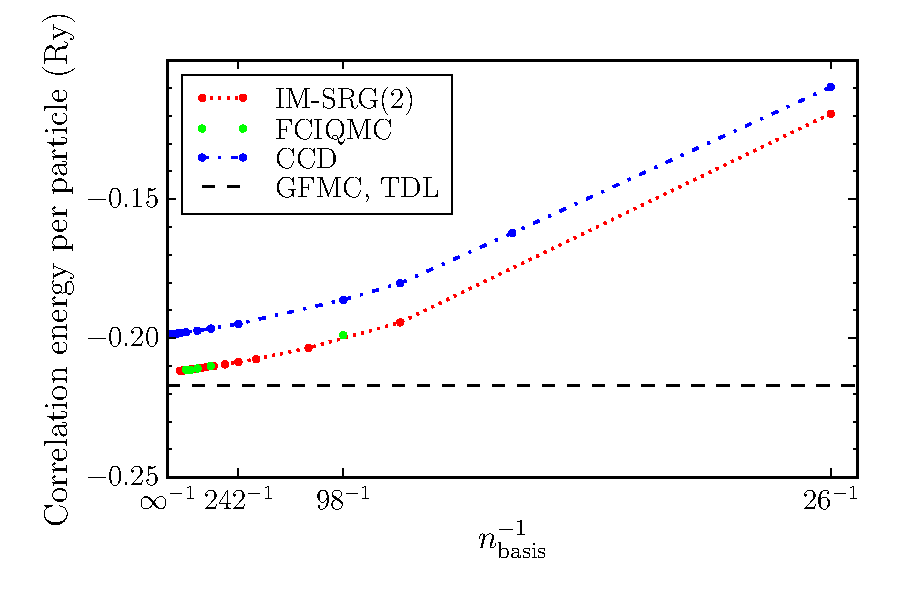
\includegraphics[width=0.4\textwidth]{figures/nOrbitsEneN10Rs10.pdf}
    \end{center}
    \caption{Correlation energy per particle as function of the number of
single-particle orbits for a ten-particle electron gas at $r_s=1.0$, using CCD, IMSRG(2) 
and FCIQMC. The IMSRG(2)
correlation energies are in excellent agreement with the almost
exact FCIQMC results. For comparison, we have marked the correlation
energy in the thermodynamic limit, as obtained by extrapolating GFMC
energies. The width of the horizontal line shows the statistical error of
the GFMC calculations.}
            \label{fig:N10}
\end{figure}


\begin{figure}[hbtp]
     \begin{center}

            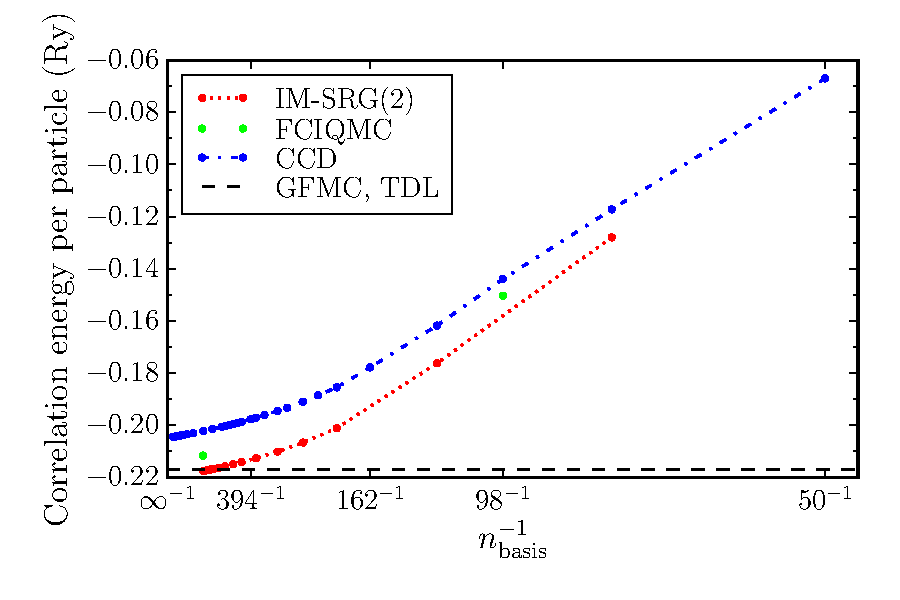
\includegraphics[width=0.4\textwidth]{figures/nOrbitsEneN26Rs10.pdf}
    \end{center}
    \caption{Correlation energy per particle as function of the number of
single-particle orbits for a 26 particle electron gas at $r_s=1.0$, using CCD, IMSRG(2) 
and FCIQMC. Here we see a larger discrepancy between the IMSRG(2) results and the FCIQMC values. 
For comparison, we have marked the correlation
energy in the thermodynamic limit, as obtained by extrapolating GFMC
energies.}
            \label{fig:N26}
\end{figure}


\begin{figure}[hbtp]
     \begin{center}

            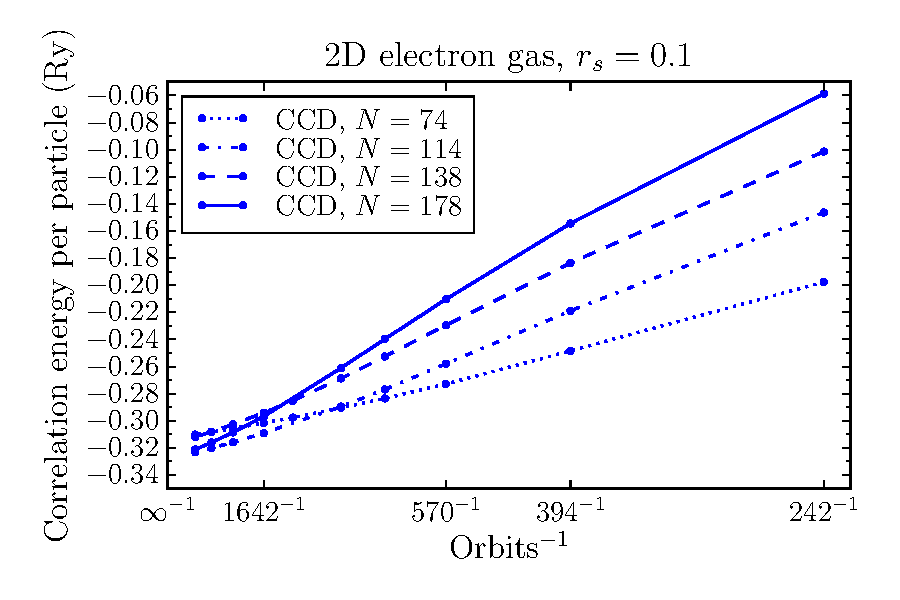
\includegraphics[width=0.4\textwidth]{figures/nOrbitsEneNRs01.pdf}
    \end{center}
    \caption{CCD correlation energy per particle as function of the number of
single-particle orbits for varying  electron numebrs $N$ $r_s=0.1$.}
            \label{fig:ccd01}
\end{figure}

\begin{figure}[hbtp]
     \begin{center}

            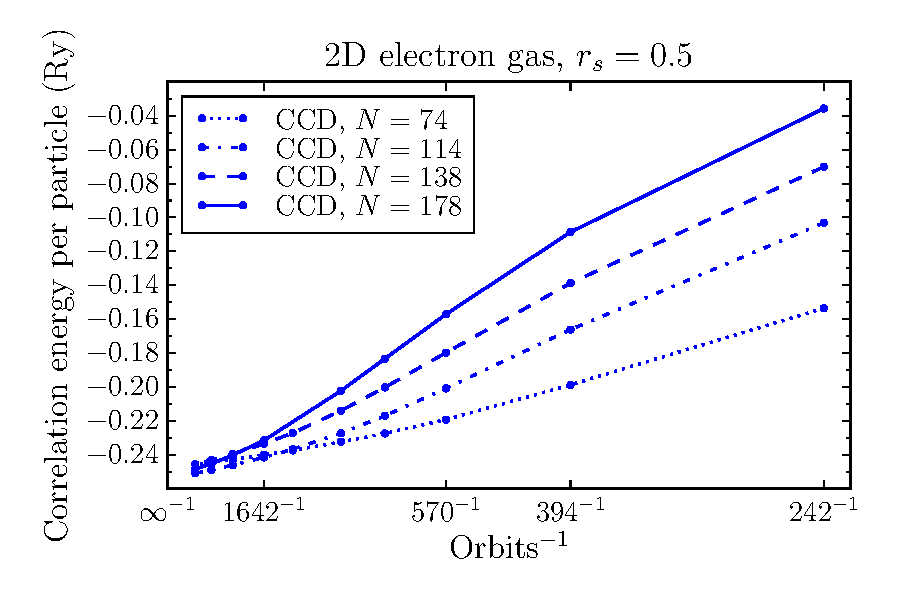
\includegraphics[width=0.4\textwidth]{figures/nOrbitsEneNRs05.pdf}
    \end{center}
    \caption{CCD correlation energy per particle as function of the number of
single-particle orbits for varying  electron numebrs $N$ $r_s=0.5$.}
            \label{fig:ccd05}
\end{figure}


\begin{figure}[hbtp]
     \begin{center}

            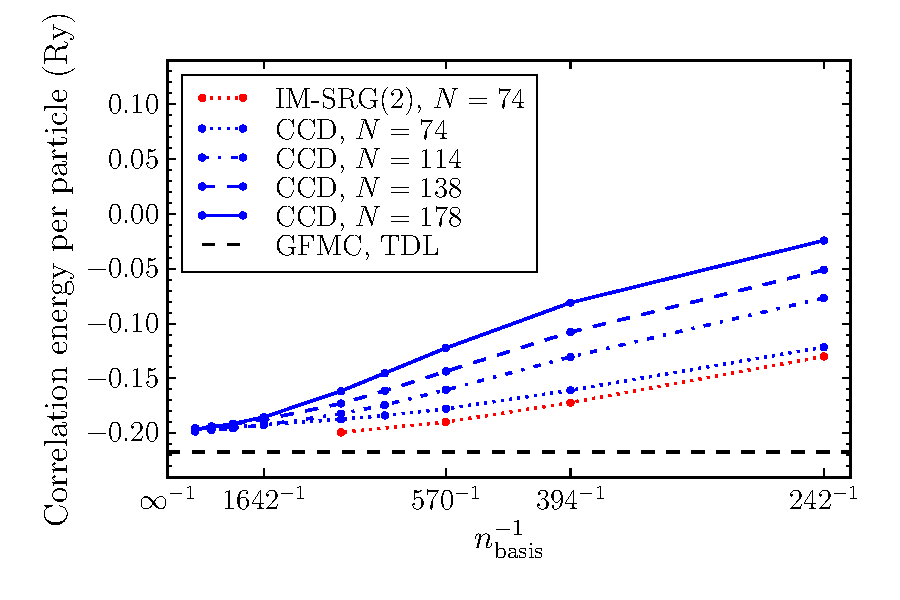
\includegraphics[width=0.4\textwidth]{figures/nOrbitsEneNRs10.pdf}
    \end{center}
    \caption{CCD correlation energy per particle as function of the number of
single-particle orbits for varying  electron numebrs $N$ $r_s=1.0$.}
            \label{fig:ccd05}
\end{figure}

\begin{figure}[hbtp]
     \begin{center}

            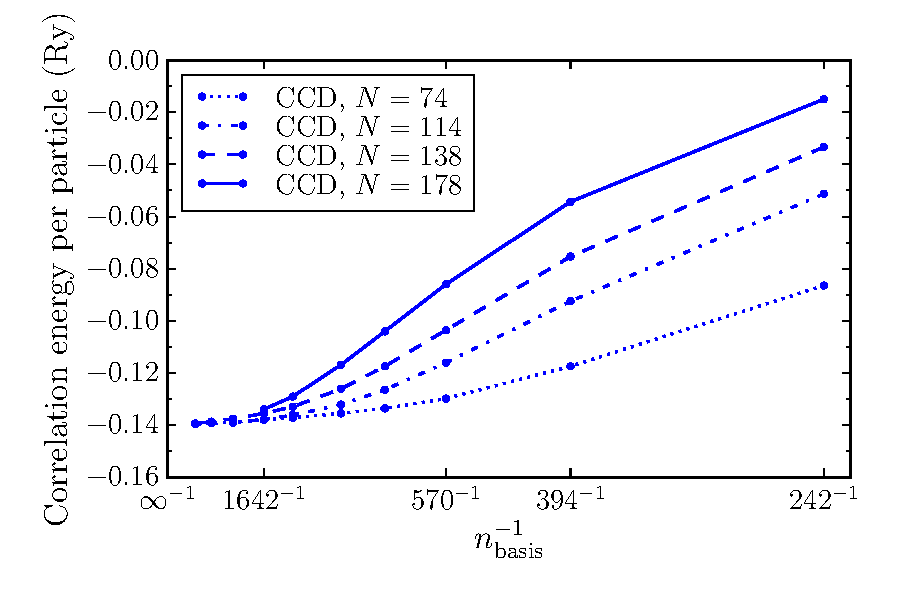
\includegraphics[width=0.4\textwidth]{figures/nOrbitsEneNRs20.pdf}
    \end{center}
    \caption{CCD correlation energy per particle as function of the number of
single-particle orbits for varying  electron numebrs $N$ $r_s=2.0$.}
            \label{fig:ccd05}
\end{figure}




\begin{align}
\frac{d E_0}{ds} &= \sum_{ia}\left( \eta_{ia}^{(1)}f_{ai} -
\eta_{ai}^{(1)}f_{ia}\right) +
\frac{1}{2}\sum_{ijab}\eta_{ijab}^{(2)}v_{abij},
\label{eq:flow1}\\
\frac{d f_{pq}}{ds}&= \sum_r \left( \eta_{pr}^{(1)}f_{rq} +
\eta_{qr}^{(1)}f_{rp}\right) + \sum_{ia}\left( 1-\hat{P}_{ia}\right)
\left( \eta_{ia}^{(1)}v_{apiq} - f_{ia}\eta_{apiq}^{(2)} \right)
\notag \\ & +\frac{1}{2} \sum_{aij} \left( 1+\hat{P}_{pq}\right)
\eta_{apij}^{(2)}v_{ijaq} + \frac{1}{2}\sum_{abi}\left(
1+\hat{P}_{pq}\right) \eta_{ipab}^{(2)}v_{abiq},
\label{eq:flow2}
\end{align}


\begin{align}
\frac{d v_{pqrs}}{ds} &= \sum_t \left( 1-\hat{P}_{pq} \right) \left(
\eta_{pt}^{(1)}v_{tqrs}-f_{pt}\eta_{tqrs}^{(2)}\right) -\sum_t \left(
1-\hat{P}_{rs} \right) \left( \eta_{tr}^{(1)} v_{pqts} - f_{tr}
\eta_{pqts}^{(2)}\right) \notag \\ & +\frac{1}{2}\sum_{ab}
\lb\eta_{pqab}^{(2)} v_{abrs} - v_{pqab}\eta_{abrs}^{(2)}\right) -
\frac{1}{2}\sum_{ij} \lb\eta_{pqij}^{(2)} v_{ijrs} -
v_{pqij}\eta_{ijrs}^{(2)}\right) \notag \\ & -\sum_{ia} \left( 1-
\hat{P}_{ia} \right) \left( 1-\hat{P}_{pq}\right) \left(
1-\hat{P}_{rs} \right) \eta_{aqis}^{(2)}v_{ipar}.
\label{eq:flow3}
\end{align}





\section{Conclusions}
\label{sec:conclusions}
%
\begin{acknowledgments}
  This work was supported by the 

\end{acknowledgments}


\bibliography{paper} \bibliographystyle{apsrev4-1}

\end{document}








  \begin{itemize}
  \item The first study of the 2D electron gas with SRG, FCIQMC, and CC  
  \item How well can the methods describe correlations?
  \item At what densities do SRG and CC break down?
  \item Theoretical explanation of breakdown?
  \item Ring and ladder approximations vs. CCD 
  \item What are differences between finite and periodic systems
    (QD vs. 2DEG)
  \item Compare 2D with finite thickness 2D+1D (or 3D?)
  \item Virial theorem (J{\o}rgen's thesis)?
  \item More ideas?
  \end{itemize}





